%
\begin{document}
	% Introduction

\chapter{Introduction} \label{chap::intro}

The exhaustion of conventional supplies of mineral and energy resources has become a rising and well known problem in the past decades. This has lead to the development of new techniques which provide the possibility to exploit more difficult-to-reach reservoirs of these resources, as well as preventing and reducing environmental costs. An important breakthrough in this matter is directional drilling, a technology that allows to drill wells with complex geometry in order to access unconventional reservoirs of energy and mineral.

Directional drilling has proven to be a successful and cost-efficient process in important applications, such as:

\begin{enumerate}[(a)]
	\item Drilling to reservoirs, which are inaccessible using conventional techniques, such as resource deposits under a city or a natural area, providing a smaller environmental and social impact (Figure~\ref{fig:app1}).
	\item Drilling relief wells to release pressure in hazardous situations when control over a well is lost. This was demonstrated at the gulf of Mexico Deepwater Horizon oil spill in 2010, when two reliefs wells where drilled in order to seal the failure (Figure~\ref{fig:app2}).
	\item If a reservoir is close to a geological fault, directional drilling can be used to drill away from the fault plane avoiding damage to the well caused by fault slippage (Figure~\ref{fig:app3}).
	\item  	Multiple wells can be drilled from the same drill rig, reducing economic and environmental costs compared to drilling processes that require to drill separate boreholes from a different rig (Figure~\ref{fig:app4}).
\end{enumerate}


\begin{figure}[ht]
	\centering
	\begin{subfigure}[b]{0.45\textwidth}
		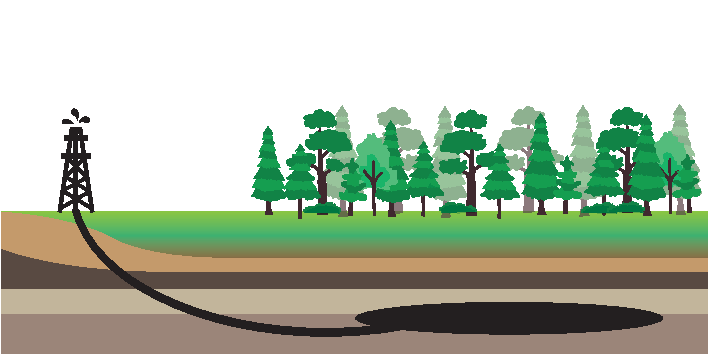
\includegraphics[width=0.9\textwidth]{img/appdd1.pdf}
		\caption{\label{fig:app1}}
	\end{subfigure}
	\begin{subfigure}[b]{0.45\textwidth}
		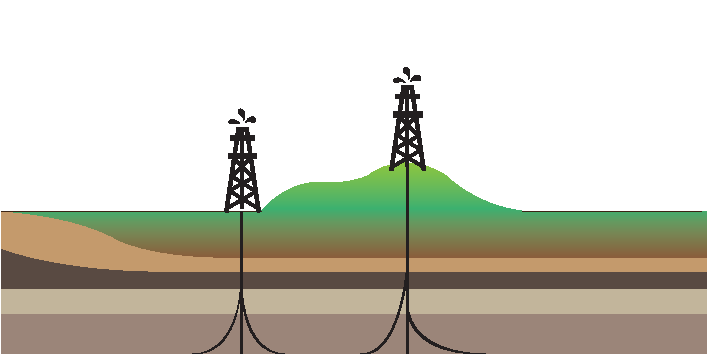
\includegraphics[width=0.9\textwidth]{img/appdd2.pdf}
		\caption{\label{fig:app2}}
	\end{subfigure}
	\begin{subfigure}[b]{0.45\textwidth}
		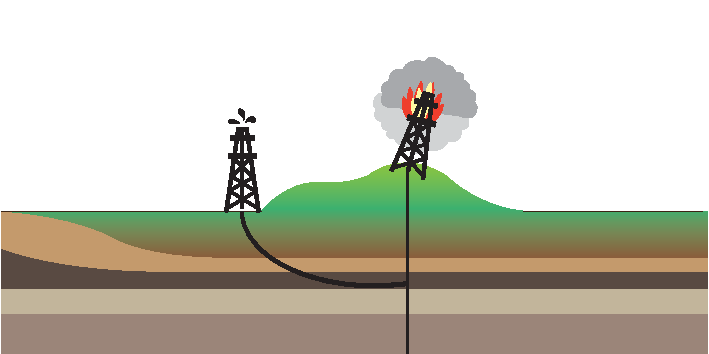
\includegraphics[width=0.9\textwidth]{img/appdd3.pdf}
		\caption{\label{fig:app3}}
	\end{subfigure}
	\begin{subfigure}[b]{0.45\textwidth}
		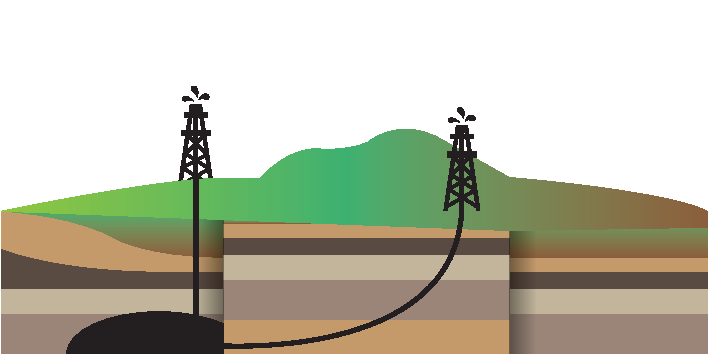
\includegraphics[width=0.9\textwidth]{img/appdd4.pdf}
		\caption{\label{fig:app4}}
	\end{subfigure}
	\caption{\label{fig:apps}Applications of directional drilling.}
\end{figure}

Figure~\ref{fig:apps} shows the different applications of directional drilling. 

In order to steer the drilling mechanism, different methods have been implemented~\cite{Downton2000}. 

Conventionally, steerable motors were used to change direction during the drilling process. This motors have two modes: rotating and sliding. In the first mode, the whole drill rotates as in conventional drilling in a straight direction. In order to change direction, the drillstring is halted and a downhole motor is used, which is powered by drilling muds in order to point the bit in the desired drilling direction, the two modes are shown in Figure~\ref{fig:drillingmodes}. This method proved to be very challenging, requiring a lot of skill from the drill operators and as the complexity of boreholes was increased the quality diminished due to the crookedness induced by the rotating mode. 



\begin{figure}[ht]\centering
	\begin{subfigure}[b]{0.15\textwidth}
		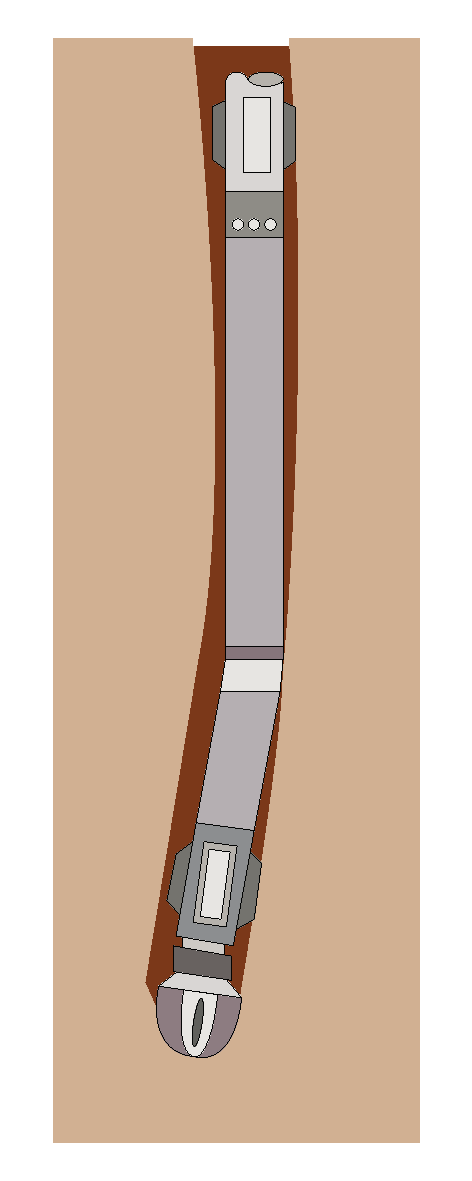
\includegraphics[width=0.9\textwidth]{img/drillingmode1.pdf}
		\caption{\label{fig:drillingmode1}Sliding.}
	\end{subfigure}
	\begin{subfigure}[b]{0.15\textwidth}
		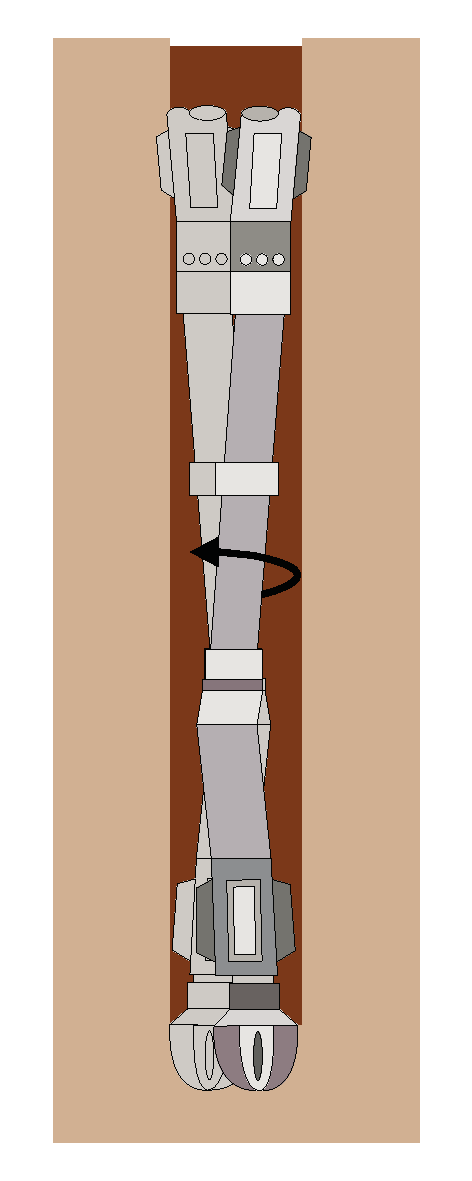
\includegraphics[width=0.9\textwidth]{img/drillingmode2.pdf}
		\caption{\label{fig:drillingmode2}Rotating.}
	\end{subfigure}
	\caption{\label{fig:drillingmodes}Drilling modes of a steerable motor.}
\end{figure}

Because of the previously mentioned issues, a new method to steer the direction of the drill was developed, namely the \acf{RSS}. This type of technology allows the drilling system to change direction while drilling, reducing borehole tortuosity, drilling time as well as increasing the \acf{ROP}.

\section{General description of the directional drilling system}
%Read ~\cite{Monsieurs2015}, ~\cite{Kremers2013}, ~\cite{Perneder2013} introductions and ~\cite{Downton2000}

A directional drilling system consists of the elements depicted in Figure~\ref{fig:directionaldrilling}. The drillsting (generally of a length in the order of kilometers) is the assembly of components from surface to bottom. Along this, power is transmitted to provide axial force and rotational speed imposed at the drill rig. For the upper part of the drillstring, the axial force (commonly known as hookload) along with its own weight, provide tension in the drillstring to prevent buckling. The \acf{BHA} constitutes the lower part of the drillstring and is usually in the order of hundreds meters long. The \acs{BHA} is in compression,  in contrast with the upper part of the drillstring, to induce an axial force transmitted to the drill bit, called weight on bit. The \acs{BHA} is commonly equipped with 3 to 5 stabilizers. 

\begin{figure}[ht]\centering
	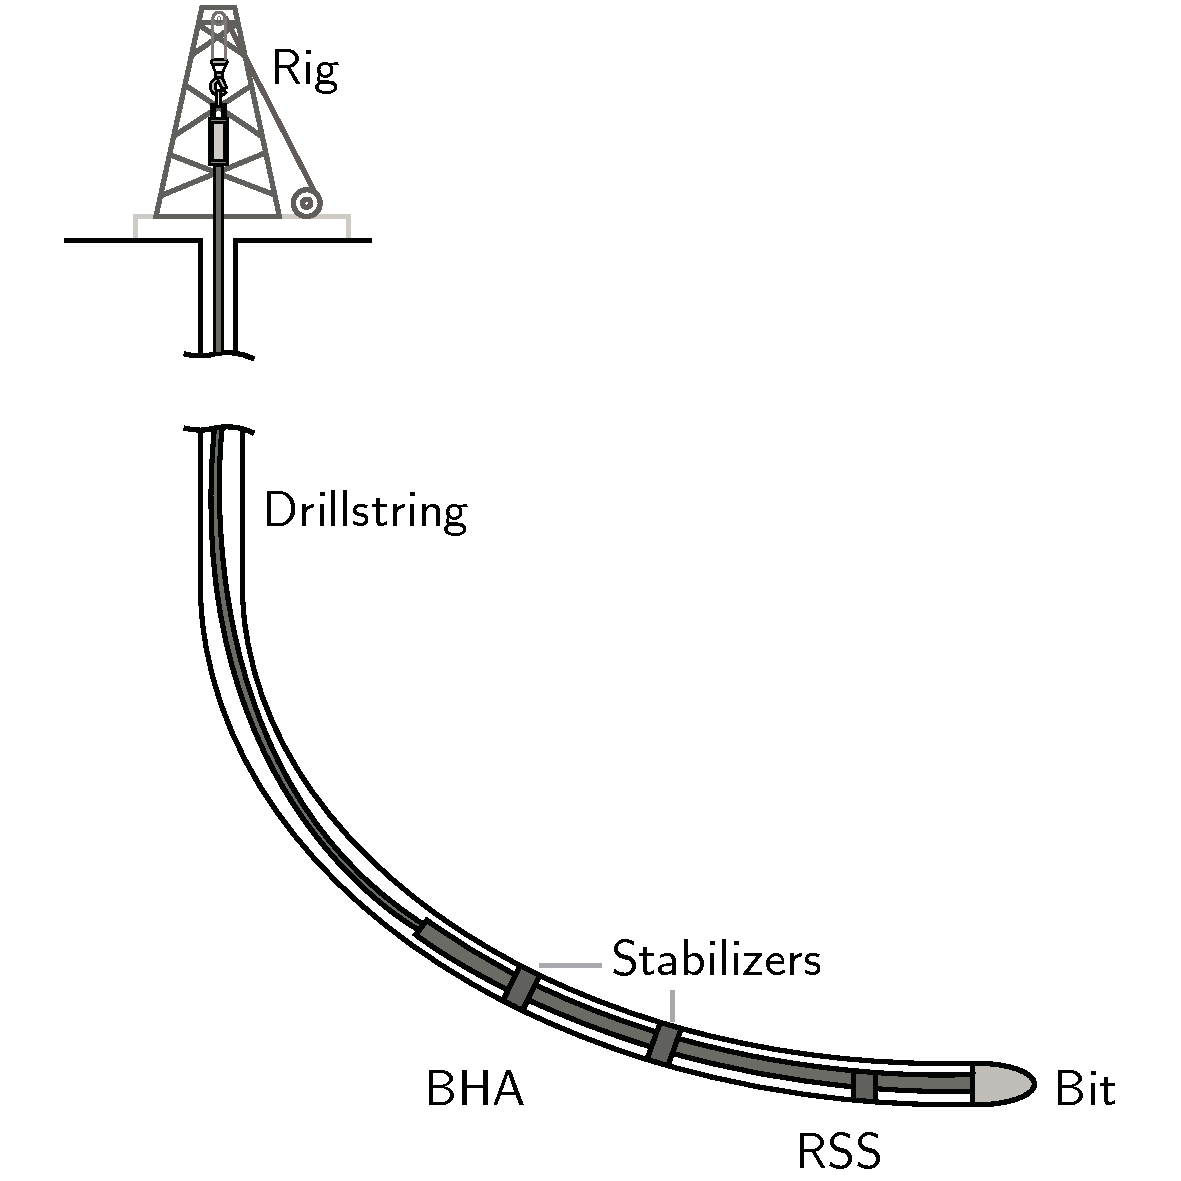
\includegraphics[width=0.4\textwidth]{img/drillingsystem.pdf}
	\caption{\label{fig:directionaldrilling}General description of a directional drilling system.}
\end{figure}

Between the first stabilizer and the bit, the previously mentioned \acs{RSS} is placed. It is equipped with mud actuators and sensors to provide inclination and azimuth control of the borehole. There exist two main types of \acs{RSS}: push-the-bit and point-the-bit. The first one applies lateral force, pushing the drillstring against the borehole using pads actuated by mud diverted with a disk valve. In point-the-bit systems, the bit is tilted relative to the rest of the tool to achieve the desired trajectory~\cite{Downton2000}. In recent years, a new type of \acs{RSS} is being researched on~\cite{Felczak2012}. This type of mechanism (called hybrid \acs{RSS}) combines the principles of point-the-bit and push-the-bit systems. Despite this, the most widely implemented type of \acs{RSS} is the push-the-bit type and its functioning is demonstrated in Figure~\ref{fig:RSS}.

\begin{figure}
	\centering
	\begin{minipage}[t]{.5\textwidth}
		\centering
		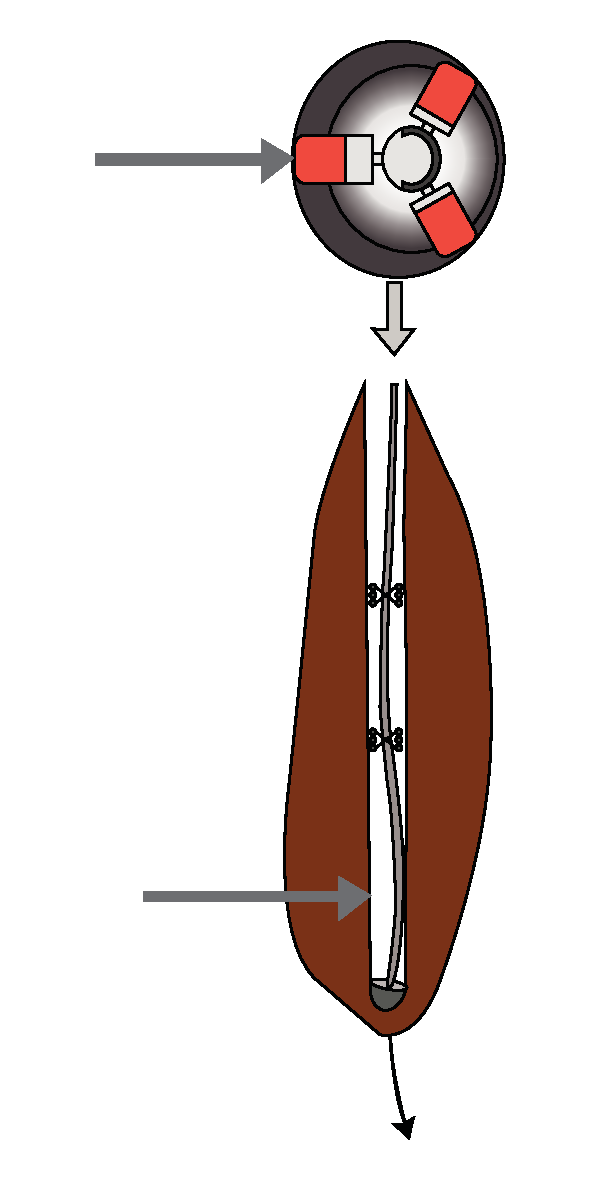
\includegraphics[width=.35\linewidth]{img/RSS.pdf}
		\captionof{figure}{RSS push-the-bit system.}
		\label{fig:RSS}
	\end{minipage}%
	\begin{minipage}[t]{.5\textwidth}
		\centering
		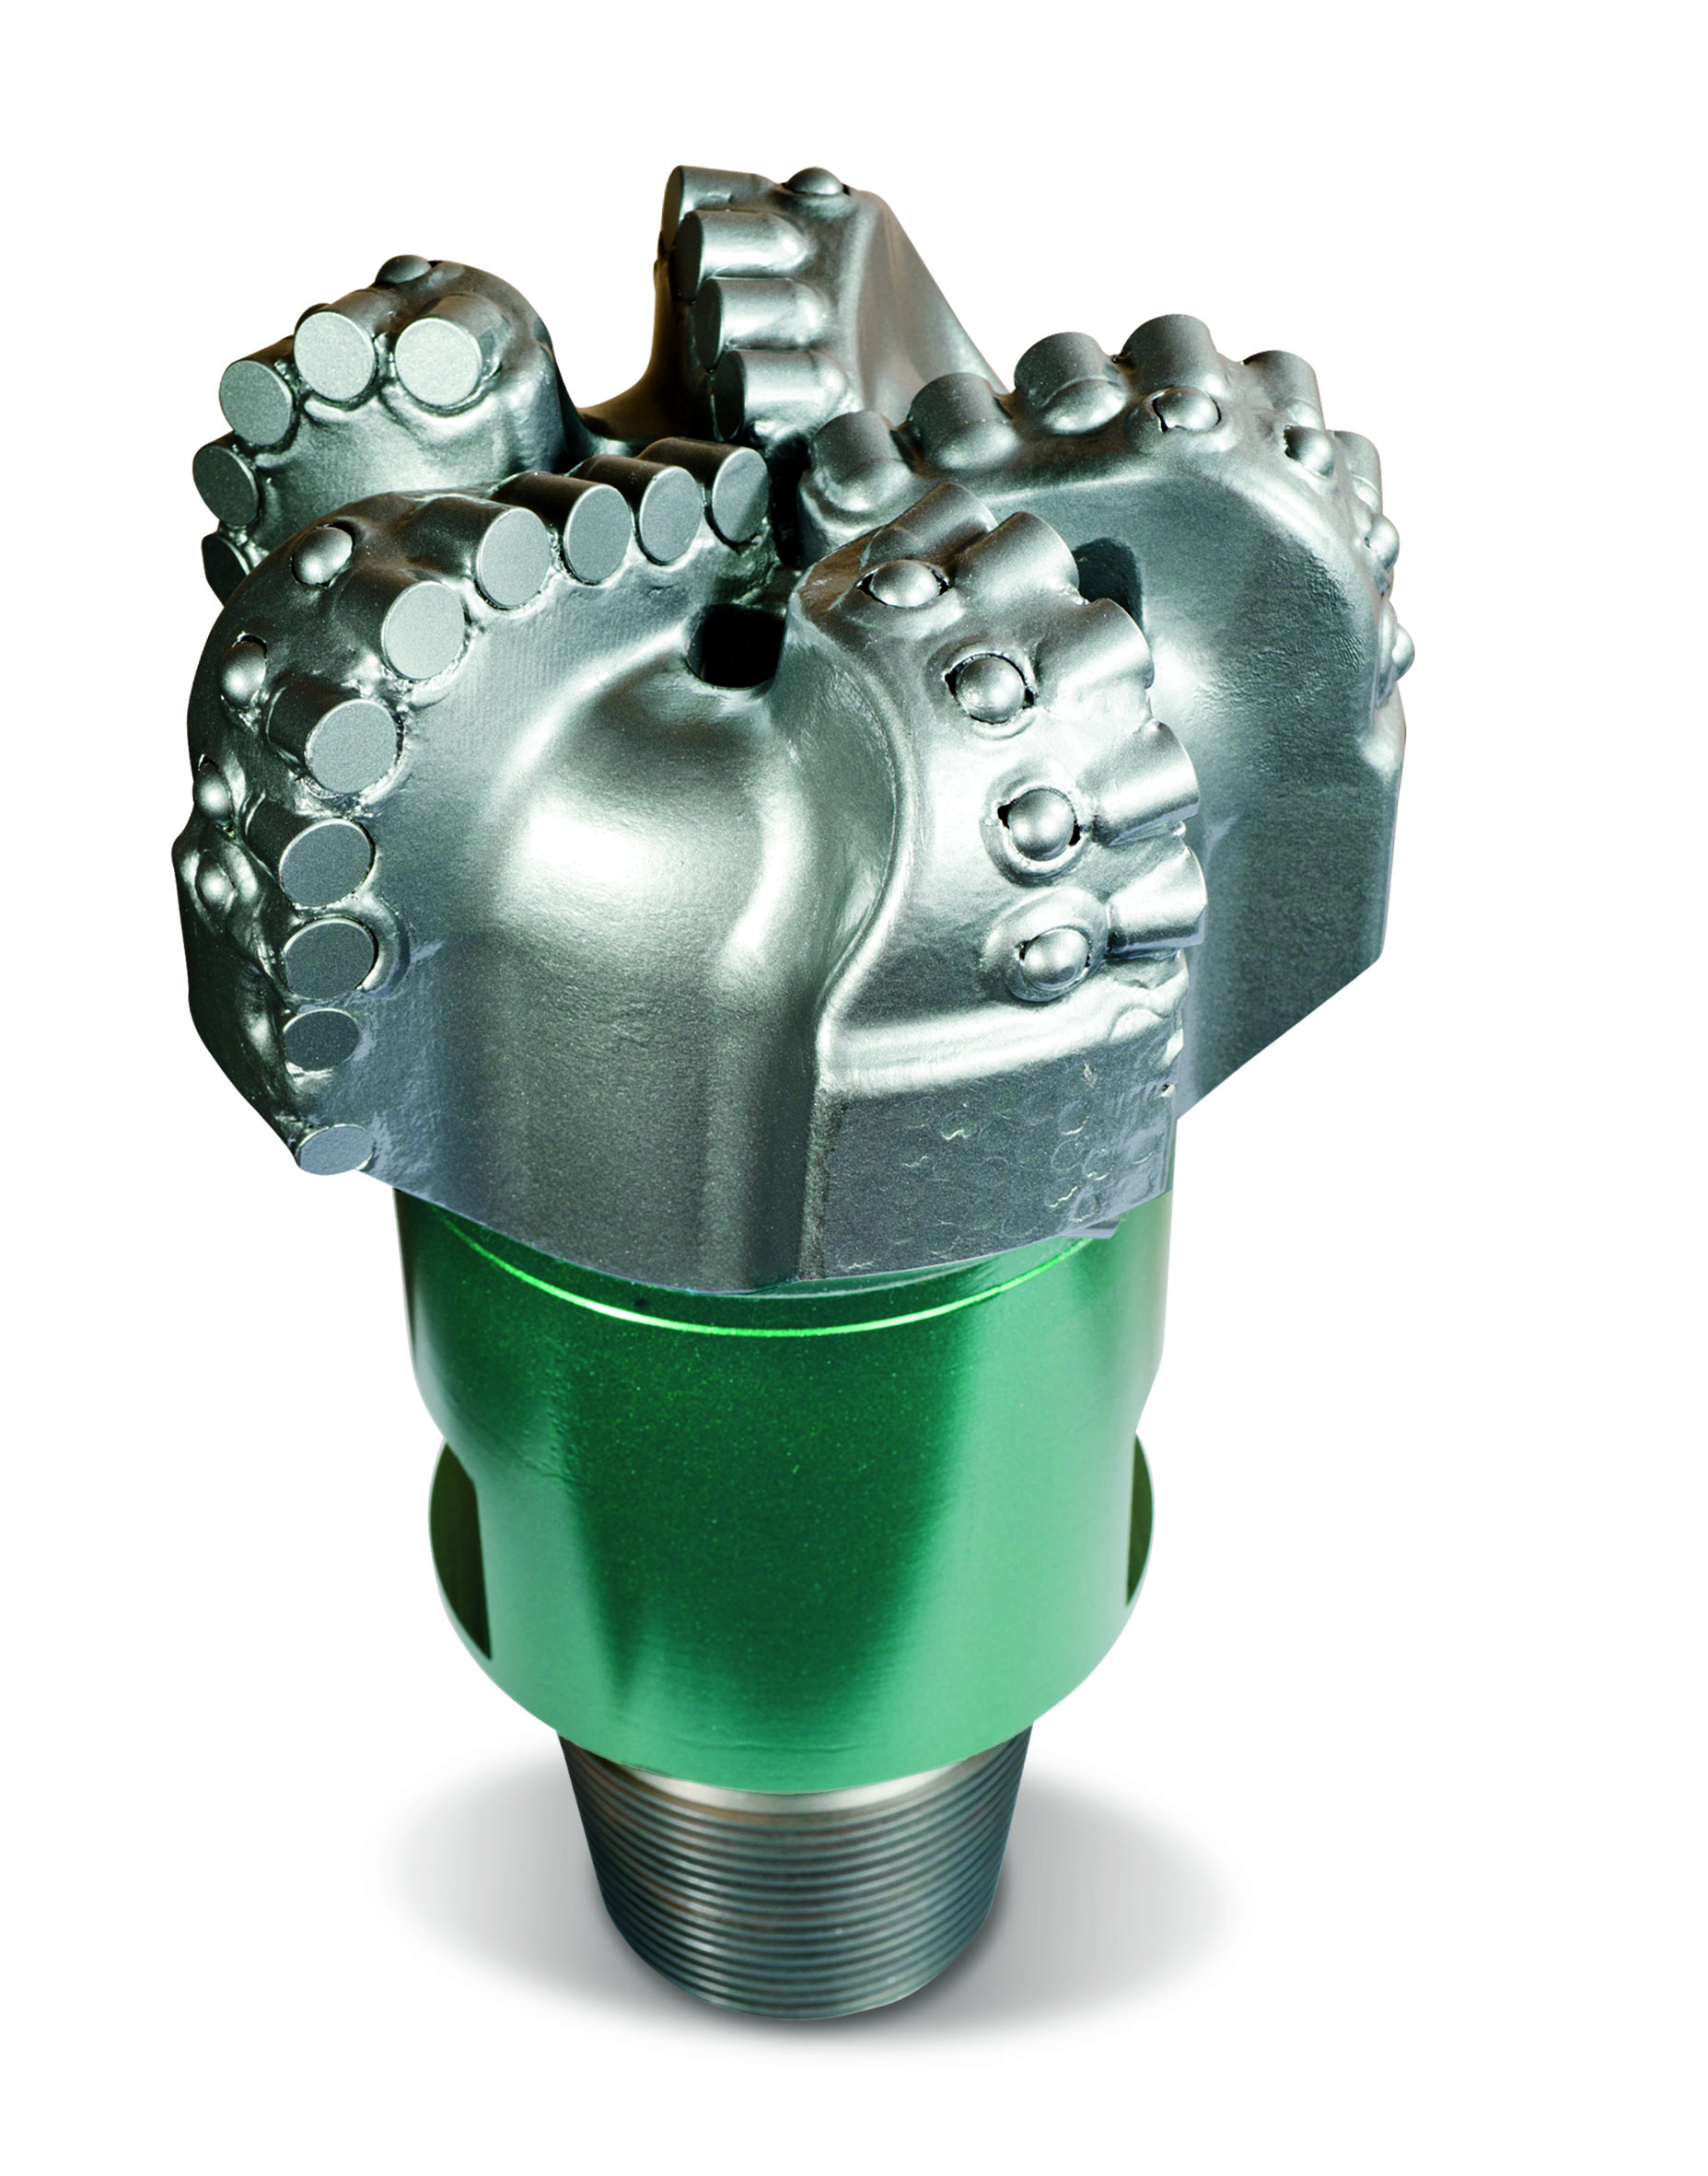
\includegraphics[width=.6\linewidth]{img/PDC-bit.pdf}
		\captionof{figure}{PDC drill bit~\cite{Bit}.}
		\label{fig:PDC}
	\end{minipage}
\end{figure}


In most cases for directional drilling, \acf{PDC} bits are used, an example of these is shown in Figure~\ref{fig:PDC}. This type of bit rotates using mud injected from the rig and it is, in particular, laterally aggressive while drilling a borehole. This last characteristic, among other causes, can produce a commonly known phenomenon called bit walk tendency, which is the natural behavior of the bit to deviate from its original path due to the lateral forces present while drilling. This effect induces the formation of spiraling patterns along the borehole walls~\cite{JulienMarckEmmanuelDetournayAndreaKuesters2014} which can be harmful to the drilling process causing:

\begin{enumerate}[(a)]
	\item An increase of frictional resistance of the borehole, which reduces the \acs{ROP}, considerably affecting drilling times.
	\item Reduced target-reach accuracy.
	\item Difficulty in the insertion of the casing after the borehole has been drilled.
	\item In a severe case, instability of the borehole evolution.
\end{enumerate} 

Reducing this borehole spiraling effect is one of the main challenges in the directional drilling industry in recent years.

\begin{figure}[ht]\centering
	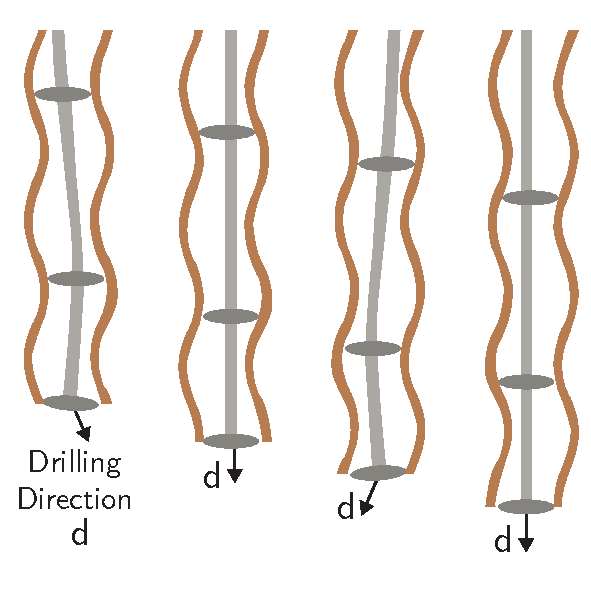
\includegraphics[width=0.3\textwidth]{img/boreholespiraling.pdf}
	\caption{\label{fig:boreholespiraling}Borehole spiraling mechanism~\cite{Marck2013}.}
\end{figure}

In addition to the \acs{RSS}, directional drilling systems nowadays are equipped with \acf{MWD} systems, that allow the driller to receive information from the downhole elements to the surface at the same time as the drilling process takes place. Current MWD systems use the fluid flowing from inside the borehole, propagating it up to the top of the drillstring, which in practice generates a slow transmission of information (at a rate of the order of 10 bits per second~\cite{Perneder2013}). 

The control process of the \acs{RSS} is generally conducted by three control loops:

\begin{enumerate}
	\item The main control loop, which sends commands for the actuation forces of the \acs{RSS} in order to steer the borehole in a desired orientation using parameterized angles.
	\item An inner control loop which translates the incoming commands of the main loop into the \acs{RSS} valve system.
	\item An outer control loop which is in charge of correcting possible deviations in Cartesian coordinates, which are generally corrected by a human operator. 
\end{enumerate}

A schematic block diagram of the three control loops is shown in Figure~\ref{fig:controlloops}. In present time, the most common practice  for \acs{RSS} type of systems is to apply constant force, expecting to obtain a constant curvature, which is generally not the case. The focus of this survey will be on the main control loop, as this is the most involved level of control when steering the systems and, furthermore, it is believed that borehole spiraling can be corrected at this loop by implementing an RSS orientation controller. 

There is not much research on control of directional drilling with a \acs{RSS}, in part because it is relatively new to the industry~\cite{Downton2000}. As a consequence of this novelty, there are still discrepancies between the models that describe it. In most situations, developed controllers are designed for two-dimensional models, for which the bit walk tendency is not taken into account. This is greatly disadvantageous, since this effect is one of the main causes of borehole spiraling.

\begin{figure}[ht]\centering
	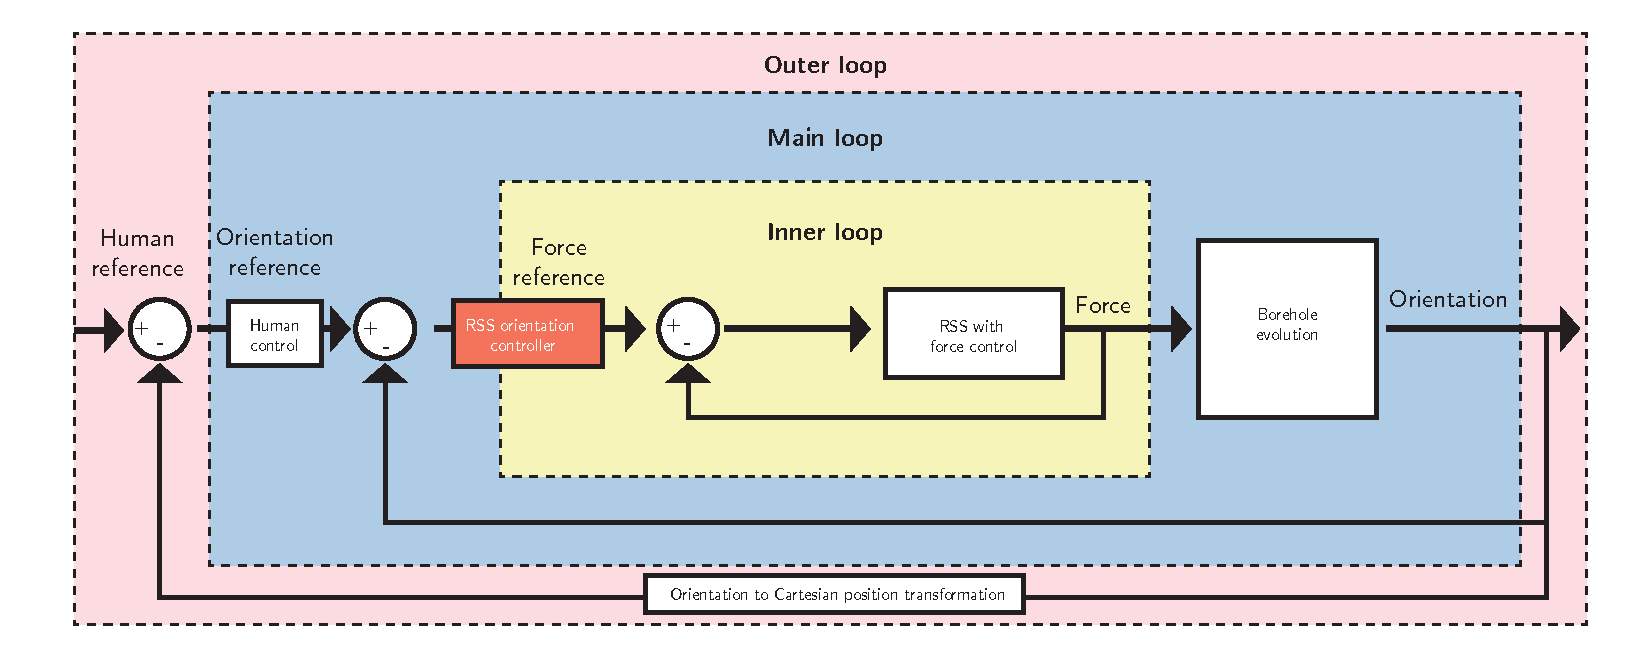
\includegraphics[width=0.8\textwidth]{img/controlloops.pdf}
	\caption{\label{fig:controlloops}Control loops of a directional drilling system.}
\end{figure}

\section{Outline of the literature survey}
The main goal of this literature survey is to provide an overview of previous works on the control of directional drilling, to ultimately assess the main challenges for this type of process and to propose a direction for the upcoming research in the author's MSc project. Since the models on which controllers are applied differ greatly from one to another, Chapter 2 will focus on the different numerical and mathematical descriptions of directional drilling. It is important to notice, that the notation for the different models varies significantly from one representation to the other. It has been chosen to keep the notation given by the authors so it can be compared to the original papers.

 Chapter 3 will go deeper into the type of controllers that have been developed for the different models, analyzing their qualities in order to choose a starting point for the upcoming research work. It is important to notice that the main challenges of directional drilling for \acs{RSS} are related to borehole quality which is, in turn, directly related to borehole spiraling. This chapter analyzes how each of the controllers tackles this problem. As before, that notation is kept the same as the one given by the authors.
 
 Chapter 4 will draw the conclusions derived from the literature survey performed in order to provide a first initial control approach for the remaining work of the thesis. Ultimately the conclusion of this survey has to be a definite proposal for a control strategy that deals with the unconsidered or inconclusive issues in previous works.
 
\end{document}
 
 


